\section{Methods}\label{sec:methods}

\subsection{Experimental Setup}\label{sec:experimental_method}

% new version
To study the dynamic sorption of TCE onto the selected building materials, we use a two-step process - one for sorption and one for desorption.
A graphic representation of this system is shown in Figure \ref{fig:js_sx_setup}.\par

In the sorption process a 7.5 by 1.27 cm stainless steel column is filled with material.
(Before filling the column, the materials had to be ground-up using a coffee grinder, except soil.
We use 2.0 g of drywall, and 1.0 g of the other materials.)
Using flow controllers, TCE is diluted in nitrogen gas to 1.12 $\mathrm{ppb_v}$ and flowed through the column at a rate of 60 mL per minute, for a pre-selected time period.
After the material has sorbed for the selected time, the column is detached and attached to the desorption system.\par

In the desorption system, the column is heated to 100 \degree C and pure nitrogen gas is flowed through the previous outlet side of the column - carrying the desorbed contaminant with it.
The now contaminated nitrogen gas is then passed through a long circular pipe, allowing the gas to cool to room temperature, and flowing into a carbon-filled stainless steel sorption column.
The sorption column is then desorbed into a gas-chromatograph fitted with a electron capture device according to the EPA TO-17 standard.\par

\begin{figure}
  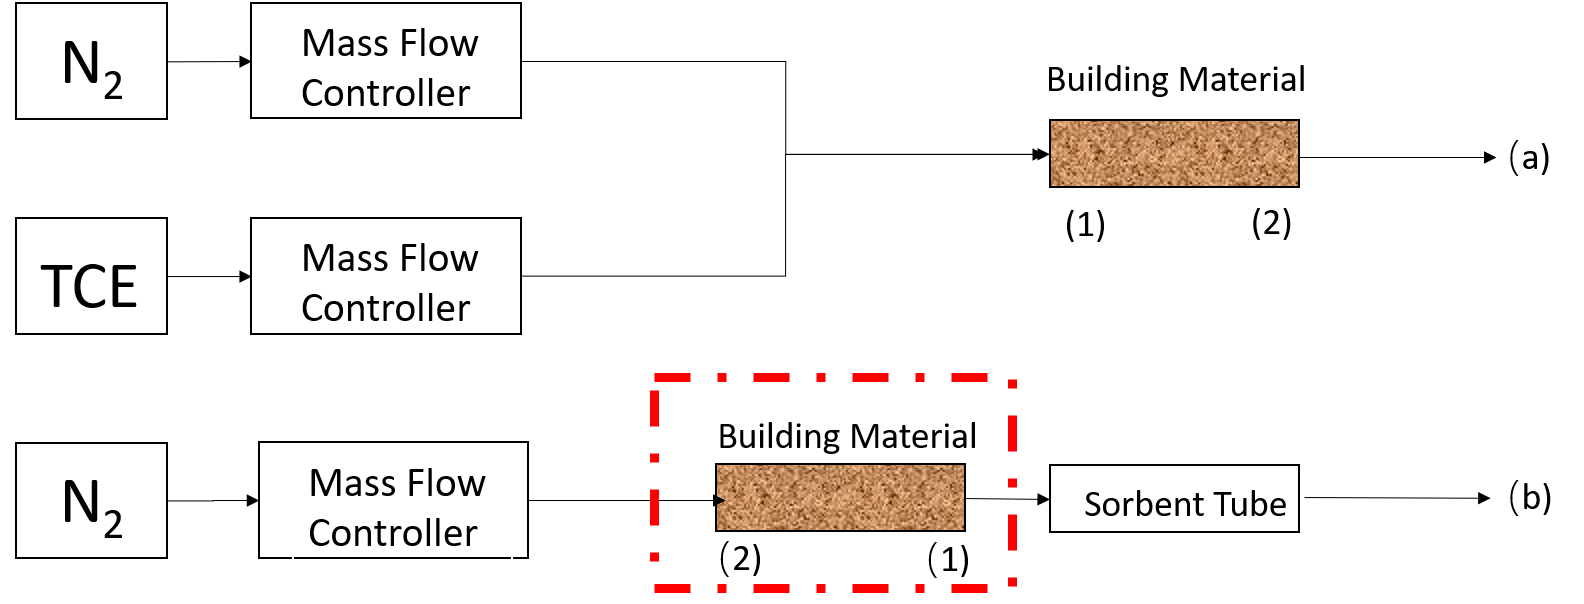
\includegraphics[width=\textwidth]{JS_SX_experiment_setup.png}
  \caption{Schematic of experimental setup.} % TODO: Shuai: Write longer description?
  \label{fig:js_sx_setup}
\end{figure}

\subsection{Numerical Model}\label{sec:model}

To investigate the role of sorption in VI, we consider VI impacted house with a 10 by 10 m footprint, with the foundation bottom located 1 m below ground surface (bgs).
The sole contaminant source is an uniformly TCE contaminated groundwater located 4 bgs, and the soil surrounding the house is assumed to homogenous and of a singular type.
All contaminant vapors are assumed to enter the house through breaches in the foundation, modeled as a 1 cm wide crack that runs along the perimeter of the house.
Finally we assume that sorption processes can occur both in the soil matrix and in the indoor environment (on various indoor materials).
Figure \ref{fig:model} shows a schematic of this model.\par

Modeling this scenario requires us to simulate a couple of physics, many of which depend and interact with each other.
The soil contains a variable moisture content and is modeled using van Genuchten's retention model\cite{van_genuchten_closed-form_1980}, which determines the effective permeability of the soil matrix and the contaminant effective diffusivity.
Darcy's Law models the gas velocity in the soil matrix, which is used to determine the advective mass transport.
Contaminant mass transport is assumed to occur through advection and diffusion, and distributed between gas, water, and sorbed onto solid phases.
The indoor air space is modeled using as a continuously stirred tank reactor (CSTR), where the reaction term determines the sorption onto/from the indoor materials.
It is important to note that the indoor environment is implicitly modeled, but instead only given by the CSTR equation; the soil domain is explicitly modeled.\par

% TODO: Make some nice figure
\begin{figure}
  %\includegraphics{}
  \caption{The vapor intrusion model. Not yet done.}
  \label{fig:model}
\end{figure}

\subsubsection{Vadose Zone Moisture Content}

Since the contaminant transport occurs through three-phased the vadose zone, it is important that we correctly account for soil moisture content and its effect on advective and diffusive transport.
In this modeled scenario, we assume that the soil moisture is at steady-state and does not change, and thus the soil moisture content is given by the retention model developed by van Genuchten\cite{van_genuchten_closed-form_1980}.\par

The van Genuchten retention model gives the soil water saturation as a function of elevation above groundwater.
In turn this gives the water and gas filled porosities, and the relative permeability of the soil matrix.
\begin{align}
  % saturation
  \mathrm{Se} &=
    \begin{cases}\label{eq:van_genuchten_saturation}
      \frac{1}{(1 + \alpha z^n)^m} & z < 0 \\
    1 & z \geq 0
    \end{cases} \\
  % soil moisture
  \theta_w &=
    \begin{cases}\label{eq:van_genuchten_soil_moisture}
      \theta_r + \mathrm{Se}(\theta_s - \theta_r) & z < 0 \\
      \theta_s & z \geq 0
    \end{cases} \\
  % relative permeability
  k_r &=
    \begin{cases}\label{eq:van_genuchten_relative_permeability}
      \mathrm{Se}^l \big[ 1 - \big( 1 - \mathrm{Se}^\frac{1}{m} \big) \big]^2 & z < 0 \\
      0 & z \geq 0
    \end{cases}
\end{align}
$\mathrm{Se}$ is the saturation, and ranges from 0 to 1, which represent completely un- to fully saturated;
$z$ is the elevation above the groundwater in meters;
$\theta_r$, $\theta_s$, $\theta_w$, and $\theta_g$ are the residual moisture content, saturated porosity (or just porosity), and water and air filled porosities respectively. All units are in volume of phase divided by the volume of soil;
$k_r$ is the relative permeability of water, which modifies the saturated permeability. This too ranges from 0 to 1, indicating completely im- and permeable respectively. $1-k_r$ gives the relative permeability of air.\par

\subsubsection{Gas Flow In The Vadose Zone}\label{sec:darcy}

The gas flow in the vadose zone is governed by a modified version of Darcy's Law.
Originally, Darcy's Law was developed to describe flow in saturated porous media, but since we're interested in flow in unsaturated media, modification is necessary.
An effective permeability that depends on the relative permeability from van Genuchten is introduced to allow for correct flow profiles in unsaturated porous media.\par
% TODO: Find a good reference for DL. Maybe one of my books?

The vapor flow continuity governing equation is given by
\begin{equation}\label{eq:darcy}
  \frac{\partial}{\partial t} (\rho \theta_s) + \nabla \cdot \rho \Big( -\frac{(1-k_r) \kappa}{\mu} \nabla p \Big) = 0
\end{equation}
Here $\rho$ is the fluid density;
$\nabla$ is the del operator;
$\kappa$ is the saturated permeability;
$\mu$ is the fluid viscosity; and $p$ is the fluid pressure.
We assume that the contaminant vapors are so dilute that the gas flow properties can be taken to be those of air, and specifically at 20 \degree C and all the transport properties may be found in Table \ref{tbl:model}.\par

\paragraph{Boundary Conditions}

To solve \eqref{eq:darcy} we assign the atmosphere boundary (see Figure \ref{fig:model}) to be at reference pressure and act as a gauge, i.e. zero pressure.
The foundation crack boundary is assigned the indoor-outdoor pressure difference value.
Remaining boundaries are no-flow boundary conditions.
\begin{align}
  &\text{Atmosphere} &p = 0 \; \mathrm{(Pa)} \\
  &\text{Foundation crack} &p = p_\mathrm{in/out} \; \mathrm{(Pa)} \\
  &\text{All other} &-\vec{n}\cdot\rho_\mathrm{air}\vec{u} = 0 \; \mathrm{(kg/(m^2\cdot s))}
\end{align}
Here $\vec{n}$ and $\vec{u}$ are the boundary normal and gas velocity vectors.

\paragraph{Initial Conditions}

For steady-state problems, the initial conditions do not influence the solution, but by necessity simply set to zero for the entire domain.
Transient simulations however, use the initial conditions that are given by the steady-state solution.\par

\subsubsection{Mass Transport In The Vadose Zone}\label{sec:mass_transport}

Contaminants in the vadose zone exist in three phases - gaseous, solved in water, and sorbed onto soil particles.
While there are three distinct phases, the water and gas phases are related via Henry's Law \eqref{eq:henrys_law}.
\begin{equation}\label{eq:henrys_law}
  c_g = K_H c_w
\end{equation}
Where $c_g$ and $c_w$ are the gas and water phase concentrations respectively in $\mathrm{mol/m^3}$;
$K_H$ is the dimensionless Henry's Law constant.\par

In this work, we consider sorption between the soil and vapor phases, as a function of the water contaminant concentration, through linear sorption \eqref{eq:linear_sorption}.
\begin{equation}\label{eq:linear_sorption}
  c_s = K_\mathrm{ads} \rho_b c_g = K_\mathrm{ads} \frac{\rho}{1-\theta_t} K_H c_w
\end{equation}
Here the $c_s$ is the solid phase concentration in $\mathrm{mol/kg}$;
$\rho_b$ is the bulk density of the soil $\mathrm{kg/m^3}$, which is given by the density $\rho$ and the total soil porosity $\theta_t$;
$K_\mathrm{ads}$ is the sorption isotherm in $\mathrm{m^3/kg}$.
Using Henry's Law and the linear isotherm we can express the total contaminant concentration in terms of the water contaminant concentration.\par

Mass transport in the vadose zone is governed by diffusion and advection and is given by \eqref{eq:mass_transport}.
\begin{equation}\label{eq:mass_transport}
  R \frac{\partial c}{\partial t} =
    \nabla \cdot[ D_\mathrm{eff} \nabla c] -
    K_H \vec{u} \cdot \nabla c
\end{equation}
The first term in \eqref{eq:mass_transport} gives the change in contaminant water concentration with respect to time, modified by the \textit{retardation factor}, $R$, which is discussed below;
The second is the effective diffusive flux which is modified by the effective diffusion coefficient $D_\mathrm{eff}$ which is also discussed below.
The third is the advective flux where $\vec{u}$ is the soil-gas velocity from Darcy's Law, which when multiplied with $K_H$ gives the gas phase concentration advective flux.\par

\paragraph{Contaminant entry into the building}

The contaminant enters the building through a combination of advection and diffusive fluxes and is given by \eqref{eq:contaminant_entry}.
\begin{equation}\label{eq:contaminant_entry}
  j_{ck} = \begin{cases}
    u_{ck} c_g - \frac{D_\mathrm{air}}{L_\mathrm{slab}} (c_{in} - c_g) & u_{ck} \geq 0 \\
    u_{ck} c_{in} - \frac{D_\mathrm{air}}{L_\mathrm{slab}} (c_{in} - c_g) & u_{ck} < 0
\end{cases}
\end{equation}
Here the $j_{ck}$ is the molar contaminant flux into the building in $\mathrm{mol/(m^2 \cdot s)}$;
$D_\mathrm{air}$ is the contaminant diffusion coefficient in pure air in $\mathrm{m^2/s}$;
$L_\mathrm{slab}$ is the thickness of the foundation slab in $\mathrm{m}$.
The flux expression changes if there is a bulk flow into the building, i.e. $u_{ck} \geq 0$, or out of the building.

\paragraph{Retardation factor}

As the contaminants are transported through the vadose zone, the partitioning between the various phases increases the contaminant residency time, retarding the transport of contaminants.
This effect is represented by $R$ which is the retardation factor \eqref{eq:retardation_factor}.
\begin{equation}\label{eq:retardation_factor}
  R = \theta_w + \theta_g K_H + \rho_b K_H K_\mathrm{ads}
\end{equation}
Here $\theta_w$, $\theta_g$ are the water and gas filled soil porosities;
$K_\mathrm{ads}$ is the solid-gas phase sorption isotherm in $\mathrm{m^3/kg}$.
The diffusive and advective transport retardation is proportional to the inverse of $R$.
\begin{align}
  D_\mathrm{retarded} &= \frac{D_\mathrm{eff}}{R} \\
  \vec{u}_\mathrm{retarded} &= \frac{\vec{u}}{R}
\end{align}
It should be noted that the soil-gas velocity, $\vec{u}$, is not retarded in of itself, but rather just the contaminant being transported through advection, giving a effective bulk velocity.\par

\paragraph{Effective diffusivity}

The effective diffusivity in the vadose zone varies with the soil moisture content, from being close to that in water when fully saturated and vice versa.
Millington-Quirk developed \eqref{eq:millington-quirk} which describes the effective diffusivity in variably saturated porous media.
\begin{equation}\label{eq:millington-quirk}
  D_\mathrm{eff} = D_\mathrm{water} \frac{\theta_w^\frac{7}{3}}{\theta_t^2} + \frac{D_\mathrm{air}}{K_H} \frac{\theta_g^\frac{7}{3}}{\theta_t^2}
\end{equation}
Where the porosity fractions are the water and gas phase tortuosity terms;
$D_\mathrm{air}$ and $D_\mathrm{water}$ are the contaminant diffusion coefficient in air and water respectively in $\mathrm{m^2/s}$.\par

\paragraph{Boundary Conditions}

A few boundary conditions are required to solve \eqref{eq:mass_transport}.
In this model, the sole contaminant source is assumed to be the homogenously contaminated groundwater, which we assume to have a fixed concentration.
The atmosphere acts as a contaminant sink, and any contaminant that makes it to this boundary is ifinitely diluted, thus this is simply a zero concentration boundary condition.
Contaminants leave the soil domain and enter the building through a combination of advective and diffusive gas phase transport.
The last boundary condition is applied to all other boundaries and is a no-flow boundary.
\begin{align}
  &\text{Groundwater} & c_w = 0 \; \mathrm{(mol/m^3)} \\
  &\text{Atmosphere} & c_w = c_{gw} \; \mathrm{(mol/m^3)} \\
  &\text{Foundation crack} & -\vec{n} \cdot \vec{N} = - \frac{j_{ck}}{K_H} \; \mathrm{(mol/(m^2 \cdot s))}\\
  &\text{All other} & -\vec{n} \cdot \vec{N} = 0 \; \mathrm{(mol/(m^2 \cdot s))}
\end{align}
$\vec{n} \cdot \vec{N}$ is the dot product between the boundary normal vector and the contaminant flux;
$j_ck$ is the contaminant vapor flux into the building.
We assume that only contaminants in the gas phase enter the building, and dividing $j_{ck}$ by $K_H$ we get proper accounting in terms of the water phase concentration.\par

\paragraph{Initial Conditions}

For a steady-state condition the initial conditions don't matter, but are set to be zero everywhere.
For transient simulations in this work, the steady-state solution is always used as an initial condition.

\subsubsection{Indoor Environment}\label{sec:indoor_environment}

The indoor air space is modeled as a continuously stirred tank reactor (CSTR) given by \eqref{eq:cstr}.
Contaminants are assumed to only enter through the foundation crack, represented by $n_\mathrm{ck}$, which is calculated by integrating the contaminant flux over the foundation crack boundary.
The product of air exchange rate, which govern how many house volumes are exchanged with the outside per time unit, and indoor air contaminant concentration gives the contaminant exit rate.
The sorption of contaminant is given by the sorption reaction term in \eqref{eq:sorption_rate} and the sorbed contaminant concentration is given by \eqref{eq:sorbed_concentration}.

\begin{align}
  V_\mathrm{bldg} \frac{\partial c_\mathrm{in}}{\partial t} &= n_\mathrm{ck} - A_e c_\mathrm{in} V_\mathrm{bldg} + r_\mathrm{sorb} V_\mathrm{mat}\label{eq:cstr} \\
  V_\mathrm{mat} \frac{\partial c_\mathrm{sorb}}{\partial t} &= -r_\mathrm{sorb} V_\mathrm{mat}\label{eq:sorbed_concentration} \\
  r_\mathrm{sorb} &= k_1 c_\mathrm{sorb} - k_2 c_\mathrm{in}\label{eq:sorption_rate}\\
  n_\mathrm{ck} &= \int_{A_{ck}} j_{ck} dA
\end{align}

Here $V_\mathrm{bldg}$ and $V_\mathrm{mat}$ are the indoor control volume and volume of indoor material in $\mathrm{m^3}$;
$c_\mathrm{in}$ and $c_\mathrm{sorb}$ are the indoor and sorbed (onto the indoor material) contaminant concentrations in $\mathrm{mol/m^3}$;
$n_\mathrm{entry}$ is the contaminant entry rate in $\mathrm{mol/s}$, which is calculated by integrating the contaminant flux $j_{ck}$ over the foundation crack area;
$r_\mathrm{sorb}$ sorption rate in $\mathrm{mol/(m^3 \cdot s)}$;
$k_1$ and $k_2$ are desorption and sorption reaction constants in $\mathrm{1/s}$.\par % TODO: Make sure this is right.

\paragraph{Fitting Kinetic Parameters}

To calculate the indoor sorption rate we need $k_1$ and $k_2$.
These values are found by solving \eqref{eq:sorption_rate} numerically and then finding the best $k_1$ and $k_2$ by fitting them to the experimental data via least square.
We use Runge-Kutta method of order 5(4) as the numerical solve, which is implemented together with the least square method in the SciPy python package\cite{jones_scipy_2011}.

% TODO: Create table of all the constants and values used
\begin{table}
  \caption{Transport properties and model parameters. To be completed.}
  \label{tbl:model}
\end{table}
